%!TEX root = ../main.tex
\section{Preliminary Testing} % (fold)
\label{sec:preliminary_testing}
In an effort to split the development into smaller, more managable parts, it was decided to initially develop the system such that it fulfills the following requirements:

\begin{itemize}
	\item The cart should be able to move with known position.
	\item Endstops on the platform should stop movement.
	\item Emergency button should stop movent.
\end{itemize}

Clearly, making the cart move is crucial in the development of the system and forms the basis for any later developments.
The latter two requirements are related to the safe operation of the platform.
It is expected that at least during development, an error may occur that causes the cart to move uncontrollably.
In such a situation the programmer should be able to completely shut off power to the motor.
The endstops will ensure that a minimum of mechanical or electrical damage is incurred on the platform in case of a cart crash.
The following paragraphs will explore what is required in order to fulfill the above requirements.
\subsection{Safety Circuitry} % (fold)
\label{sub:safety_circuitry}
Safety first.
A safety system should, whenever possible, be isolated from the remaining system.
That is, it should depend on non of the remaining circuitry or programming.
Usually, if it can at all be avoided, no programming should be involved in determining a safety condition.
With this in mind, the safety system for this platform should be designed in such a way that, when activated, it will cut power to the motors.
In order to more easily identify the cause of the fault, the remaining electronics should remain operational to maintain the current program status.
\\~\\
Creating the endstops can be done in a multitude of ways.
In this project three approaches were considered:
\paragraph{Mechanical Switch:} % (fold)
\label{par:mechanical_switch}
The simplest form of switch is the mechanical switch.
The switch should be mounted in such a way that the cart would move into the switch, therefore activating it.
This approach is not without issues.
Firstly, the simplest mounting solution would require the switch to be mounted in the direct path of the cart.
If the cart is traveling at full speed it is unlikely that the cart would stop before crashing into the switching mechanism, potentially damaging it.
A switch mounted in this fashion would need to be rather robust.
Some other mounting solutions could be thought of that do not suffer from this problem, especially if a flexible microswitch is used.
These types of switches can be fragile and may not be sufficiently durable, considering the usecase.
All mechanical switches have one drawback in common: they are mechanical.
Generally, mechanical items wear out over time and require maintainance or replacement.
% paragraph mechanical_switch (end)
\paragraph{Hall Effect Sensor:} % (fold)
\label{par:hall_effect_sensor}
This type of sensor measures magnetic fields and produces a voltage proportional to the strength of the field.
By placing a small neodymium magnet on the cart and mounting a hall effect sensor on the rail in such a way that the coincide would allow for detecting when the cart is above the sensor.
If the sensor is combined with a schmitt-trigger circuit the output could be a binary result, either the endstop is reached or it is not.
Using this method requires that a magnet is placed on the cart itself and that a sensor is mounted to the rail.
It should be noted that accelerating rather strong magnetic fields back and forth on the platform may not be the least electrically noisy solution one could think of.
Magnetic fields are also wide, meaning that the cart would "sneak up on" the threshold.
This requires some amount of calibration to determine the correct distance between sensor and magnet, which may not be mechanically simple to determine. 
% paragraph hall_effect_sensor (end)
\paragraph{Infrared Transceiver:} % (fold)
\label{par:infrared_transceiver}
This type of device is a combined LED and infrared sensor.
The LED is optimised for emitting infrared light, or radiation (IR), and the sensor for sensing it.
The LED emits IR outward from the device which, when an object is placed in front of it, will bounce off the object and be caught by the sensor.
As with the hall effect sensor, this type of device produces a voltage output proportional to the amount of IR being sensed and as such a schmitt-trigger circuit would also be benficial in this case.
With this sensor type it is important to realise that the LED will not be the only emitter of IR in the vicinity.
Any type of lamp will emit IR, especially glowbulbs (of which there are few left, luckily) but also sunlight contains some amount of IR.
When using this sensor the circuit should be designed in such a way that only the effect of the IR radiated back on the sensor will trigger the circuit.
The sensor should be mounted immediately below the cart so as to maximize the radiated IR and therefore the signal strength.
% paragraph infrared_transceiver (end)
\\~\\
While all of the above have their drawbacks, it was decided to use the infrared transceiver.
This sensor allows the greatest reliability while being reasonably simple to mount on the platform in that it requires no modification to the cart.
\\~\\
In addition to the endstops, also an emergency button, preferably red, should be able to cut power to the motors.
It may be that additional safety features are added later.
In order to minimize the amount of circuitry, all safety features will trip the same circuit.
\thomas{Add circuit showing the safety relay}
On figure \ref{fig:relay_circuit} is shown the safety circuitry.
A relay is mounted in series with the supply rail for the motor.
The default state for this relay should be \texttt{off}.
Then, in order to switch the system to the \texttt{on} state, the relay should be closed.
Should power to the relay coil ever fail i.e. something in the system has broken, power to the motor is cut off.
Since the relay is in series with the motor, it should also be capable of carrying the full design current, 80A.
One relay that fulfills these requirements is the.
\\~\\
The driver circuit for the relay is activated only when all safety conditions are off.
If at any point any of the safety conditions are tripped, the driver circuit shuts down, releasing the relay and turning off power to the motor.
Designing the safety circuit in this manner ensures that the system cannot be started or will shut down if any wires or components in the safety circuit break.

% subsection safety_circuitry (end)
\subsection{Power Board} % (fold)
\label{sub:power_board}
It is necessary to device some form of driving circuitry for the motor driving the timing belt.
On the platform is a Maxon 148867 Brushed DC Motor.
This is a 150W motor with a nominal current of 6A and a stall current of 80A.
Clearly, the system should under normal use not come anywhere close to stalling the motor but considering the use case, experimentation with control from students, it may be beneficial to design the circuitry such that it can withstand being stalled, for at least a short period of time.
In order to reach this goal, it is necessary to size the components for at least some amount above 80A continuous.
The \texttt{IPP045N10N3} MOSFET \cite{mosfet} is a 100V/100A MOSFET.
It is made in the standard TO-220 housing.
This housing allows for easy mounting of a heatsink and due to its wide application, there are many shapes and sizes to choose from.
Table \ref{tab:mosfetparameters} holds a list of the relevant parameters.

\begin{table}[tb]
	\centering
	\begin{tabular}{|r|c|c|c|}
	\hline
		\textbf{Parameter} & \textbf{Min} & \textbf{Typ} & \textbf{Max} \\
	\hline
		$V_{\text{th}}$ [V] & 2 & 2.7 & 3.5 \\
	\hline
		$R_{\text{ds(on)}}$ [m$\Omega$]& - & 3.6 & 4.2 \\
	\hline
		$Q_\text{g}$ [nC] & - & 88 & 117 \\
	\hline
		$I_\text{d}$ [A] & - & 100 & - \\
	\hline
		$V_{\text{ds}}$ [V] & 100 & - & - \\
	\hline
	\end{tabular}
	\caption{Relevant parameters of the IPP045N10N3 MOSFET \cite{mosfet} chosen for the full-bridge.
	Here, \vth is the gate threshold voltage, \ron is the drain-source on resistance, \qg is the total gate charge, \id is the maximum continuous drain current and \vds is the minimum guaranteed drain-source breakdown voltage.}
	\label{tab:mosfetparameters}
\end{table}

It should be noted that even though \vth is maximum 3.5V, this is not enough to fully open the MOSFET.
Rather, this voltage is where the MOSFET will start to conduct.
Figure \ref{fig:mosfettransfercharacteristic} reveals that the MOSFET is not fully conducting until \vgs $>4.5$V.

\begin{figure}[H]
	\centering
	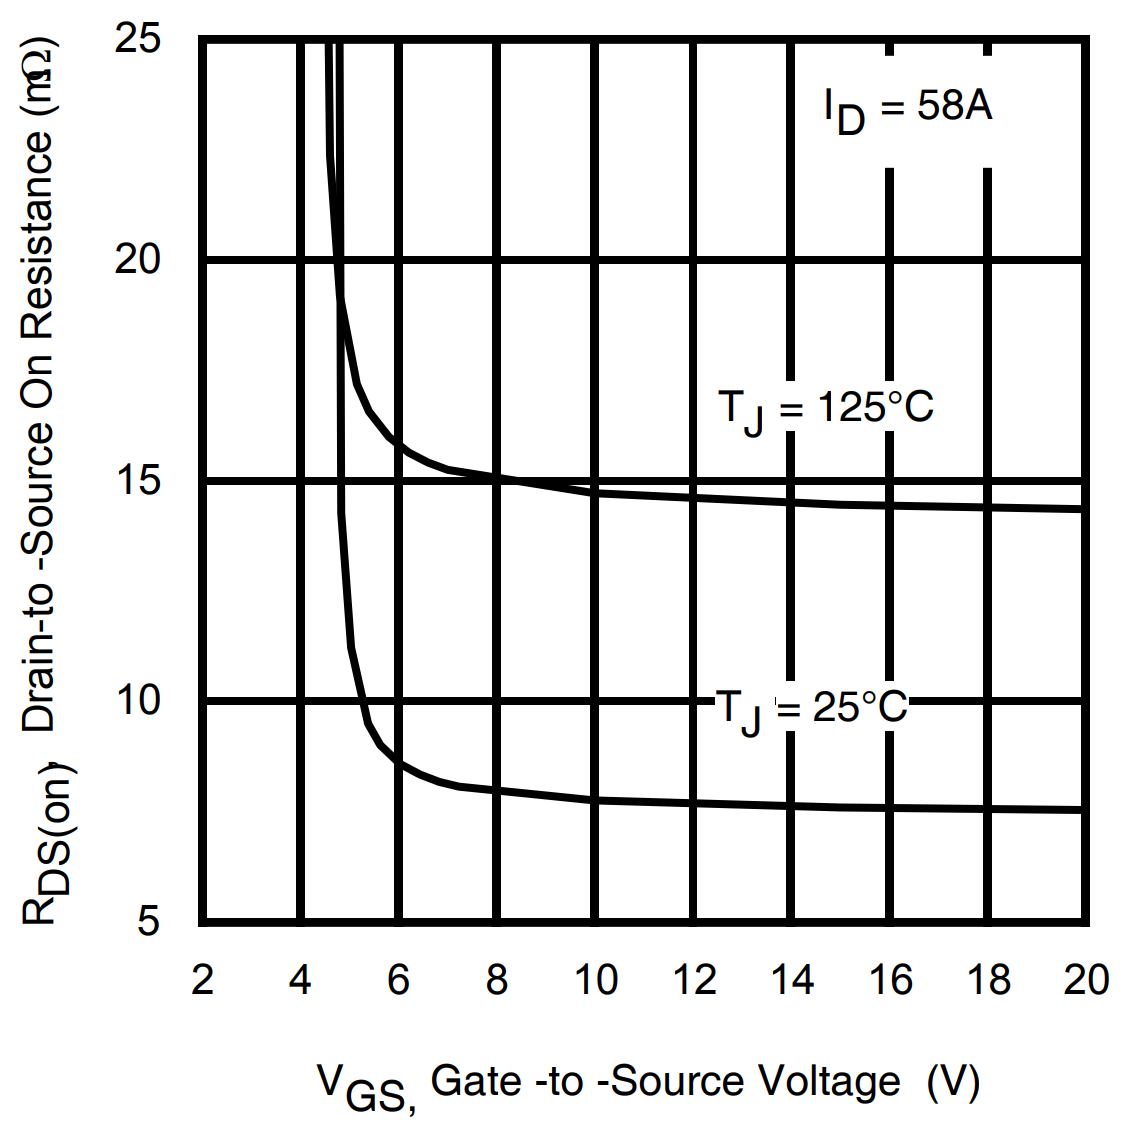
\includegraphics[width=.5\linewidth]{graphics/mosfet_transfer_characteristic}
	\caption{Transfer characteristic of the IPP045N10N3 as per the datasheet.
	Inspecting the graph reveals that the maximum \id of 100A is reached at \vgs$\approx4.5\rightarrow4.75$V.}
	\label{fig:mosfettransfercharacteristic}
\end{figure}

The motor should be able to move in both directions so an h-bridge, or full-bridge is required.
By properly switching the MOSFETs in the circuit on and off the average voltage across the motor can be controlled and therefore also the speed and direction of the motor, see \ref{sec:hbridge} for more details.
\\~\\
\thomas{Insert reference to note on full-bridge drive}
Having chosen a MOSFET for the full-bridge, some form of driver must be designed for the full-bridge.
For this task, ready-made full-bridge drivers exist on the market that incorporate all of the electronics required to generate the driving signals, requiring only a PWM signal from the designer.
In order to choose one, a few parameters must be fulfilled.

\begin{itemize}
	\item \textbf{Output Current:} The amount of current necessary to properly drive the MOSFET.
	This value depends on the switching frequency of the application, the gate-to-source voltage ($V_{gs}$) and the total gate charge of the MOSFET.
	\item \textbf{Driving Voltage:} In order to ensure that the MOSFET is turned on quickly and fully the driver should be able to supply a voltage well above the gate threshold of the MOSFET.
	\item \textbf{High-Side Drive Capabilities:} The high side MOSFET of the full-bridge is referenced not to ground, but to $V_{\text{cc}}$.
	This means that in order to switch on this MOSFET $V_{\text{gs}}$ must be at least $V_{\text{cc}}+V_{\text{th}}$ where $V_{\text{th}}$ is the gate threshold voltage of the MOSFET.
	This is bootstrapping and is explained in more detail in section \ref{sec:bootstrap}.
	\item \textbf{Shoot-Through Protection and Deadtime:} Due to the structure of the full-bridge it is important that two MOSFETs on the same half-bridge are never on at the same time as this would result in a short from $V_{\text{cc}}$ to ground.
	This is resolved with a combination of deadtime (a delay where no MOSFET is on) and a logic table that ensures that an illegal switch combination can never happen.
\end{itemize}

The HIP4081AIBZ \cite{driver} full-bridge driver meets all of the above requirements.
It can supply up to 2.5A on the output pins with a voltage approximately 1V below \vcc, well above the required \vth.
Since the motor should, preferably, be driven outside the audible frequency range, it was chosen to set the switching frequency at 22kHz.
This frequency was chosen over an even higher frequency because increasing the frequency also increases the switching losses.
At this frequency there is $\frac{1}{22000}\approx45\mu$S per cycle. 
Well within this time the gate should be fully opened.
Since:

\begin{equation}
	I = C\frac{\text{dv}}{\text{dt}} \quad\Rightarrow\quad \text{dt} = C\frac{\text{dv}}{I}
\end{equation}
\thomas{Is this the correct way of calculating it?}

Accounting for various voltage drops it is assumed that \vgs is 10V, a rough estimate of the time to open the gate completely can be found as:

\begin{equation}
	\text{dt} = 117\cdot10^{-9}\frac{10}{2.5}\approx0.47\mu\text{S}
\end{equation}

This time is approximately 100 times shorter than the allotted time frame.
The component also has floating drive circuitry, meaning that by referencing the high-side driver to source of the high-side MOSFET, the driver can be made to output a voltage higher than \vcc.
This does require a few external components for the bootstrapping.
The choice of these components and a more in depth explanation of the procedure is given in section \ref{ssub:bootstrap_circuit}.
Finally, the component has a user-programmable dead time and shoot-through protection. 

HIP4081AIBZ - Full-bridge driver - (ISL83202)

IPP045N10N3 - Mosfet

choice of VGS, 8V - show graph of transfer characteristics of mosfet, high due to uncertainty.





\subsubsection{Bootstrap Circuit}
\label{ssub:bootstrap_circuit}
\missingfigure{Put in a bootstrap circuit and make a couple of references to it, when it makes sense.}
The chosen gate driver has floating drive circuitry for the high side MOSFETS, but needs a bootstrap circuit for providing the higher voltage. 
A standard bootstrap circuits consists of a diode, a capacitor and a resistor to limit initial charging current to the capacitor. 
The advantage of using a bootstrap circuit to supply a high voltage for the floating drive is that it is very simple. 
The disadvantage is that it sets a limit for the maximum and minimum duty cycle as the bootstrap capacitor needs to be charged fully in each period.
The bootstrap circuitry for this project will be designed to have a maximum duty cycle for the higher MOSFETS of 95\%, thus meaning that the charging of the bootstrap capacitor should take no longer than 5\% of a period.  

The bootstrap diode needs to have a fast recovery time, preferably below 100 ns \cite{bootstrap_infineon}, to minimize the energy fed back to the supply from the bootstrap capacitor.
\texttt{US1M-E3} was chosen as it has a reverse recovery time of 75 ns and comes in SMD packaging. 
It allows for a maximum average forward current of 1 A and a maximum forward voltage drop of 1.7 V.
\mikkel{Kildehenvisning til datasheet?}
Determining the values for the bootstrap capacitor was done using the calculations shown in \cite{bootstrap_ON}.
The maximum allowed voltage drop across the bootstrap capacitor during \texttt{on} time needs to be determined: 
\begin{equation}
\Delta V_{boot} = V_{DD} - V_{F} - V_{GSMIN}
\end{equation}
Where $\Delta V_{boot}$ is the voltage drop across the bootstrap capacitor during \texttt{on} time, $V_{DD}$ is the supply voltage, $V_F$ is the forward voltage drop across the diode and $V_{GSMIN}$ is the minimum wanted \texttt{gate-source} voltage.
$V_{GSMIN}$ was chosen to 8 V to to ensure a high enough gate voltage to turn on the MOSFETS. 
The chosen MOSFETS have a maximum gate threshold voltage of 3.5 V. 
Inserting the values yields the maximum allowed value of $\Delta V_{boot}$:
\begin{equation}
\Delta V_{boot} = 12 - 1.7 - 8 = 2.3 V	
\end{equation}

The total charge that needs to be supplied from the bootstrap capacitor is the gate charge of the MOSFET and quiescent and leakage currents in the \texttt{on} time:
\begin{equation}
	Q_{total} = Q_{gate} + Q_{ls} + (I_{lkgs} + I_{qbs} + I_{lk} + I_{lkdiode}) \cdot t_{on}
	\label{eq:charge_total}
\end{equation}
Where $I_{lkgs}$ is the gate-source leakage current, $I_{qbs}$ is the gate driver quiescent current, $I_{lk}$ is the gate driver leakage current, $I_{lkdiode}$ is the diode leakage current, $ t_{on}$ is the \texttt{on} time and $Q_{ls}$ is the charge required by the internal level shifter in the gate driver.
\begin{table}[h]
\centering
\begin{tabular}{|l|l|l|l|l|l|l|}
 \hline
 $Q_{gate}$ 	& $Q_{ls}$ 	& $I_{lkgs}$ 	& $I_{qbs}$ 		& $I_{lk}$ 			& $I_{lkdiode}$ 	& $t_{on}$ 		\\ 	\hline
 $117$ [nC]		& $3$ [nC]	& $100$ [nA]	&$-30$ [$\mu$A]		& $1$ [$\mu$A]		& $1$ [nA]			& $43$ [$\mu$S]	\\ 	\hline
\end{tabular}
\caption{Parameter values used in equation \ref{eq:charge_total}. $I_{qbs}$ and $I_{lk}$ are found in the gate driver data sheet. $Q_{ls}$ is set to 3nC for all high voltage gate drivers \cite{bootstrap_ON}. $I_{lkgs}$ and $Q_{gate}$ are MOSFET data sheet values and $I_{lkdiode}$  is a diode data sheet value. $t_{on}$ is calculated using 95\% dutycycle and 22kHz switching.}
\label{tab:bootstrap_parameter}
\end{table}
$t_{on}$ can be calculated knowing that the worst case duty cycle for the high side MOSFET is 95\% and the switching frequency is 22 kHz.
Inserting the values, shown in \ref{tab:bootstrap_parameter}, yields the minimum charge value of the capacitor:
\begin{equation}
	Q_{total} = 119 [nC]
\end{equation}

The minimum value of the bootstrap capacitor can now be calculated:
\begin{equation}
	C_{boot} = \frac{Q_{total}}{\Delta V_{boot}} = \frac{119}{2.3} = 51.6 [nC]
\end{equation}
A ceramic capacitor will be used as it has a negligible leakage current. 
Looking for SMD ceramic capacitors it was found that in the range of the found minimum value is 56, 68, 82 and 100 [nF].
56 [nF] is, in theory, a big enough capacitor for the circuit, but a bigger capacitor is an advantage as $\Delta V_{boot}$ will then decrease.
When increasing the size of the capacitor it should be noted that the initial charge current will become larger.
It was therefore chosen to use a 100 [nF] ceramic capacitor.

The initial charge current to the capacitor needs to be limited in order not to exceed the maximum ratings of the diode.
Therefore a resistor is put in series with the diode.
The resistor value should not be too big as the voltage drop across it is subtracted from the bootstrap capacitor voltage.
A 1 $\Omega$ resistor was chosen. In this setting, the maximum current through this component is 12 A.
\mikkel{Do we have a 1 ohm resistor SMD?}
This is clearly above the maximum average forward current of the diode, but the diode can withstand a 8.3 ms single half sine-wave of maximum 30 A \cite{diode_ds}.
The charging of a capacitor is approximately finished after 5 time constants
\mikkel{MANGLER KILDE!!! Denne er måske OK \url{http://www.electronics-tutorials.ws/rc/rc_1.html}}
\begin{equation}
T_{charge,init} = 5\cdot \tau = 5\cdot (R \cdot C) = 0.5 \mu S 
\end{equation}
Meaning that the diode can be exposed to a maximum of 12A for $0.5 \mu S $, which is well below the absolute maximum rating.
It should also be noted that bootstrap capacitor needs at least $0.5 \mu S $ for the initial charging.
\mikkel{In the application note they state that they include a 400ns bootstrap}


Lastly it should be calculated what the maximum allowed duty cycle for the high side MOSFETS are in this configuration, using the found components.
The time it takes to charge the capacitor the energy that is used in each period is:
\begin{equation}
	T_{charge,period} = 5\cdot \tau = 5\cdot (R \cdot C_{boot}) = 5\cdot (1 \cdot  51.6 \cdot 10^{-9}) = 258 nS 
\end{equation}
The 258 nS are equivalent to 0.6\% duty cycle and the maximum duty cycle for the high side MOSFETS is thus 99.4\%.

% subsection power_board (end)
% section preliminary_testing (end)
